\documentclass[11pt,a4paper]{article}
% ==========================================================
%  Common preamble for the General Relativity documents
%  (IMAPP M1, Université Clermont Auvergne)
% ==========================================================
\usepackage[utf8]{inputenc}
\usepackage[T1]{fontenc}
\usepackage{lmodern}
\usepackage[english]{babel}
\usepackage[a4paper,margin=2.4cm,headheight=14pt]{geometry}
\usepackage{amsmath,amssymb,amsthm,mathtools}
\usepackage{bm}
\usepackage{enumitem}
\usepackage{booktabs}
\usepackage{array}
\usepackage{xcolor}
\usepackage{graphicx}
\usepackage{fancyhdr}
\usepackage{tikz}
\usetikzlibrary{arrows.meta,calc,decorations.pathmorphing,decorations.markings,patterns,shapes.geometric,positioning,3d,intersections}
\usepackage{pgfplots}
\pgfplotsset{compat=1.18}
\usepackage[most]{tcolorbox}
\usepackage[colorlinks=true,linkcolor=blue!50!black,citecolor=blue!50!black,urlcolor=blue!50!black]{hyperref}
\usepackage[capitalise,noabbrev]{cleveref}
\usepackage{caption}
\captionsetup{font=small,labelfont=bf}

\allowdisplaybreaks
\setlength{\parindent}{0pt}
\setlength{\parskip}{0.55em}
\numberwithin{equation}{section}

% ---------- colours ----------
\definecolor{defcol}{RGB}{0,90,160}
\definecolor{thmcol}{RGB}{160,40,40}
\definecolor{remcol}{RGB}{90,90,90}
\definecolor{excol}{RGB}{0,120,60}
\definecolor{warncol}{RGB}{200,110,0}

% ---------- boxes ----------
\tcbset{boxbase/.style={enhanced,breakable,sharp corners=south,boxrule=0.6pt,
    left=6pt,right=6pt,top=4pt,bottom=4pt,fonttitle=\bfseries,
    before skip=8pt,after skip=8pt}}
\newtcbtheorem[number within=section]{definition}{Definition}{boxbase,
    colback=defcol!4,colframe=defcol!70!black}{def}
\newtcbtheorem[use counter from=definition]{theorem}{Theorem}{boxbase,
    colback=thmcol!4,colframe=thmcol!70!black}{thm}
\newtcbtheorem[use counter from=definition]{proposition}{Proposition}{boxbase,
    colback=thmcol!4,colframe=thmcol!70!black}{prop}
\newtcbtheorem[use counter from=definition]{example}{Example}{boxbase,
    colback=excol!4,colframe=excol!70!black}{ex}
\newtcbtheorem[use counter from=definition]{exercise}{Exercise}{boxbase,
    colback=excol!4,colframe=excol!70!black}{exc}

\newtcolorbox{keyresult}[1][]{enhanced,breakable,colback=yellow!8,colframe=orange!70!black,
    boxrule=0.8pt,left=6pt,right=6pt,top=4pt,bottom=4pt,fonttitle=\bfseries,
    title={#1},before skip=8pt,after skip=8pt}
\newtcolorbox{remarkbox}[1][Remark]{enhanced,breakable,colback=remcol!5,colframe=remcol!70,
    boxrule=0.4pt,left=6pt,right=6pt,top=3pt,bottom=3pt,fonttitle=\bfseries\small,
    title={#1},before skip=6pt,after skip=6pt}
\newtcolorbox{warningbox}[1][Warning]{enhanced,breakable,colback=warncol!6,colframe=warncol!80!black,
    boxrule=0.6pt,left=6pt,right=6pt,top=3pt,bottom=3pt,fonttitle=\bfseries\small,
    title={#1},before skip=6pt,after skip=6pt}

\theoremstyle{remark}
\newtheorem*{proofsketch}{Proof sketch}

% ---------- macros ----------
\newcommand{\dd}{\mathrm{d}}
\newcommand{\pd}{\partial}
\newcommand{\R}{\mathbb{R}}
\newcommand{\M}{\mathcal{M}}
\newcommand{\Ga}[3]{\Gamma^{#1}{}_{#2#3}}
\newcommand{\Riem}[4]{R^{#1}{}_{#2#3#4}}
\newcommand{\tr}{\operatorname{tr}}
\newcommand{\sgn}{\operatorname{sgn}}
\newcommand{\GN}{G_{\mathrm N}}
\newcommand{\rs}{r_{\mathrm s}}
\newcommand{\eq}[1]{\begin{align}#1\end{align}}
\renewcommand{\Box}{\square}
\renewcommand{\vec}[1]{\bm{#1}}
\newcommand{\order}[1]{\mathcal{O}\!\left(#1\right)}
\newcommand{\half}{\tfrac12}

\usepackage{cancel}
\numberwithin{equation}{subsection}

\newtcolorbox{problem}[1]{enhanced,breakable,colback=blue!3,colframe=defcol!70!black,
  boxrule=0.6pt,left=6pt,right=6pt,top=4pt,bottom=4pt,fonttitle=\bfseries,title={#1},before skip=10pt,after skip=6pt}
\newenvironment{solution}{\par\noindent\textbf{\textcolor{excol!70!black}{Solution.}}\ }{\hfill$\blacksquare$\par\medskip}
\newcommand{\added}[1]{{\color{teal!60!black}#1}}

\pagestyle{fancy}
\fancyhf{}
\fancyhead[L]{\small\nouppercase{\leftmark}}
\fancyhead[R]{\small General Relativity --- Problems and Solutions}
\fancyfoot[C]{\thepage}

\title{\Huge\bfseries General Relativity\\[0.4em]
\Large Problem Sheets and Complete Solutions\\[1em]
\large IMAPP Master (M1) --- Université Clermont Auvergne}
\author{Problems by A.~Goudelis (LPCA, 2025);\\ solutions transcribed from the handwritten ones, completed and expanded}
\date{}

\begin{document}
\maketitle
\thispagestyle{empty}

\noindent The problem statements are reproduced from the four official problem sheets. The solutions follow the handwritten solutions; wherever these were sketched, left to the reader (``do it!'') or incomplete, the missing steps have been added; \textcolor{teal!60!black}{text in this colour marks material that is not in the handwritten solutions (completions, extra checks and remarks)}. Conventions: signature $(+,-,-,-)$; $\pd_\mu\equiv\pd/\pd x^\mu$; the Einstein summation convention is used throughout. References to ``the lecture notes'' are to the companion document \emph{General Relativity --- Complete Lecture Notes}.

\tableofcontents
\newpage

% =====================================================================
\section{Problem sheet 1: Tensors and index technology}
% =====================================================================

\subsection*{Reminder}
Under a general coordinate transformation $x\to x'(x)$, the components of a $(p,q)$ tensor transform as
\[
  T'^{\mu_1\dots\mu_p}{}_{\nu_1\dots\nu_q}=\frac{\pd x'^{\mu_1}}{\pd x^{\alpha_1}}\cdots\frac{\pd x'^{\mu_p}}{\pd x^{\alpha_p}}\frac{\pd x^{\beta_1}}{\pd x'^{\nu_1}}\cdots\frac{\pd x^{\beta_q}}{\pd x'^{\nu_q}}T^{\alpha_1\dots\alpha_p}{}_{\beta_1\dots\beta_q},
  \qquad\frac{\pd x'^\mu}{\pd x^\alpha}\frac{\pd x^\alpha}{\pd x'^\nu}=\delta^\mu{}_\nu .
\]

\subsection{Exercise 1: (anti)symmetry is preserved}
\begin{problem}{Exercise 1.1}
Consider a $(2,0)$ tensor $t^{\mu\nu}$ which is antisymmetric, i.e.\ $t^{\mu\nu}=-t^{\nu\mu}$. Show that the property of antisymmetry is preserved under general coordinate transformations. Show the same for a symmetric tensor. From this exercise we deduce that (anti-)symmetry is a fundamental property of tensors.
\end{problem}
\begin{solution}
The components of a $(2,0)$ tensor transform as
\[
  t'^{\mu\nu}=\frac{\pd x'^\mu}{\pd x^\alpha}\frac{\pd x'^\nu}{\pd x^\beta}t^{\alpha\beta}
  \overset{(\ast)}{=}-\frac{\pd x'^\mu}{\pd x^\alpha}\frac{\pd x'^\nu}{\pd x^\beta}t^{\beta\alpha}
  =-\frac{\pd x'^\nu}{\pd x^\beta}\frac{\pd x'^\mu}{\pd x^\alpha}t^{\beta\alpha}=-t'^{\nu\mu},
\]
where in $(\ast)$ we used that $t$ is antisymmetric, and in the last step we recognised the transformation law of $t'^{\nu\mu}$ (the Jacobian factors are just numbers, so their order is irrelevant; $\alpha,\beta$ are dummy indices). Antisymmetry persists in all coordinate systems.

For a symmetric tensor, $t^{\alpha\beta}=+t^{\beta\alpha}$, the same steps without the minus sign give $t'^{\mu\nu}=t'^{\nu\mu}$. The same argument applies to any pair of indices of the same type (both upper or both lower) of any tensor.
\end{solution}
\added{Remark: (anti)symmetry under the exchange of an upper and a lower index, $T^\mu{}_\nu=T_\nu{}^\mu$, is not a coordinate-independent notion unless a metric is used to relate the two positions.}

\subsection{Exercise 2: symmetric $\times$ antisymmetric}
\begin{problem}{Exercise 1.2}
Consider two general $(2,0)$ and $(0,2)$ tensors $t$ and $r$, respectively, and assume that $t$ is symmetric and $r$ is antisymmetric. Show that their scalar product vanishes.
\end{problem}
\begin{solution}
We have $t^{\alpha\beta}=t^{\beta\alpha}$ and $r_{\alpha\beta}=-r_{\beta\alpha}$. Then
\[
  t^{\alpha\beta}r_{\alpha\beta}=t^{\beta\alpha}(-r_{\beta\alpha})=-t^{\beta\alpha}r_{\beta\alpha}=-t^{\alpha\beta}r_{\alpha\beta},
\]
where in the last step, since $\alpha,\beta$ are just dummy (contracted) indices, we relabelled $\alpha\leftrightarrow\beta$. Hence $2t^{\alpha\beta}r_{\alpha\beta}=0$, i.e.\ $t^{\alpha\beta}r_{\alpha\beta}=0$.
\end{solution}

\subsection{Exercise 3: transforming the components of a tensor}
\begin{problem}{Exercise 1.3}
Consider a $(2,0)$ tensor field $T$ with components which, in some coordinate system $\{x^i\}$ of $\R^2$, read $T^{11}=1$, $T^{12}=1$, $T^{21}=-1$ and $T^{22}=2$.
\begin{enumerate}[label=\alph*)]
\item Find the components $T'^{ij}$ of $T$ in the coordinate system $\{x'^i\}$, which is connected with the $\{x^i\}$ system through
\[
  x'^1=(x^1)^2\neq0,\qquad x'^2=x^1x^2 .
\]
\item Compute the values of the components $T'^{ij}$ at the point which corresponds to $(x^1,x^2)=(1,-2)$.
\end{enumerate}
\end{problem}
\begin{solution}
\textbf{a)} Since $T$ is a $(2,0)$ tensor field, its components transform as $T'^{ij}=\frac{\pd x'^i}{\pd x^\alpha}\frac{\pd x'^j}{\pd x^\beta}T^{\alpha\beta}$. The Jacobian matrix $J^i{}_\alpha=\pd x'^i/\pd x^\alpha$ is
\[
  J=\begin{pmatrix}\frac{\pd x'^1}{\pd x^1}&\frac{\pd x'^1}{\pd x^2}\\[1ex]\frac{\pd x'^2}{\pd x^1}&\frac{\pd x'^2}{\pd x^2}\end{pmatrix}
  =\begin{pmatrix}2x^1&0\\ x^2&x^1\end{pmatrix},
\]
which is invertible since $\det J=2(x^1)^2\neq0$. In matrix form the transformation law reads $T'=J\,T\,J^T$. Component by component:
\begin{align*}
  T'^{11}&=\frac{\pd x'^1}{\pd x^1}\frac{\pd x'^1}{\pd x^1}T^{11}+\frac{\pd x'^1}{\pd x^1}\frac{\pd x'^1}{\pd x^2}T^{12}+\frac{\pd x'^1}{\pd x^2}\frac{\pd x'^1}{\pd x^1}T^{21}+\frac{\pd x'^1}{\pd x^2}\frac{\pd x'^1}{\pd x^2}T^{22}\\
  &=(2x^1)(2x^1)\cdot1+(2x^1)\cdot0\cdot1+0\cdot(2x^1)\cdot(-1)+0\cdot0\cdot2=4(x^1)^2,\\[1ex]
  T'^{12}&=\frac{\pd x'^1}{\pd x^\alpha}\frac{\pd x'^2}{\pd x^\beta}T^{\alpha\beta}=2x^1\big(x^2T^{11}+x^1T^{12}\big)=2x^1\big(x^2+x^1\big)=2x^1x^2+2(x^1)^2,\\[1ex]
  T'^{21}&=\frac{\pd x'^2}{\pd x^\alpha}\frac{\pd x'^1}{\pd x^\beta}T^{\alpha\beta}=\big(x^2T^{11}+x^1T^{21}\big)2x^1=2x^1\big(x^2-x^1\big)=2x^1x^2-2(x^1)^2,\\[1ex]
  T'^{22}&=\frac{\pd x'^2}{\pd x^\alpha}\frac{\pd x'^2}{\pd x^\beta}T^{\alpha\beta}=(x^2)^2T^{11}+x^2x^1T^{12}+x^1x^2T^{21}+(x^1)^2T^{22}\\
  &=(x^2)^2+x^1x^2-x^1x^2+2(x^1)^2=2(x^1)^2+(x^2)^2 .
\end{align*}
(For $T'^{12}$ and $T'^{21}$ we used $\pd x'^1/\pd x^2=0$, which kills all terms with $\beta=2$, resp.\ $\alpha=2$, in the factor of $x'^1$.)

\textbf{b)} By substituting $(x^1,x^2)=(1,-2)$ we find
\begin{gather*}
  T'^{11}(1,-2)=4,\qquad T'^{12}(1,-2)=-4+2=-2,\\ T'^{21}(1,-2)=-4-2=-6,\qquad T'^{22}(1,-2)=2+4=6 .
\end{gather*}
\added{Check: the antisymmetric part $\frac12(T^{12}-T^{21})=1$ transforms as $\det J\times1=2(x^1)^2$; indeed $\frac12(T'^{12}-T'^{21})=2(x^1)^2$. The symmetric part stays symmetric, as shown in Exercise 1.}
\end{solution}

\subsection{Exercise 4: contraction of a $(2,3)$ tensor}
\begin{problem}{Exercise 1.4}
Assume a $(2,3)$ tensor $t$ with components $t^{ij}{}_{klm}$. Show that the object $s$ with components $s_k\equiv t^{ij}{}_{kij}$ is a covector.
\end{problem}
\begin{solution}
Since $t^{ij}{}_{klm}$ is a $(2,3)$ tensor, its components transform under coordinate transformations as
\[
  t'^{ij}{}_{k\ell m}=\frac{\pd x'^i}{\pd x^\alpha}\frac{\pd x'^j}{\pd x^\beta}\frac{\pd x^\gamma}{\pd x'^k}\frac{\pd x^\delta}{\pd x'^\ell}\frac{\pd x^\epsilon}{\pd x'^m}\,t^{\alpha\beta}{}_{\gamma\delta\epsilon}.
\]
Setting $\ell=i$, $m=j$ (and summing), we obtain
\[
  t'^{ij}{}_{kij}=\underbrace{\Big(\frac{\pd x'^i}{\pd x^\alpha}\frac{\pd x^\delta}{\pd x'^i}\Big)}_{=\delta^\delta{}_\alpha}\underbrace{\Big(\frac{\pd x'^j}{\pd x^\beta}\frac{\pd x^\epsilon}{\pd x'^j}\Big)}_{=\delta^\epsilon{}_\beta}\frac{\pd x^\gamma}{\pd x'^k}t^{\alpha\beta}{}_{\gamma\delta\epsilon}
  =\frac{\pd x^\gamma}{\pd x'^k}\delta^\delta{}_\alpha\delta^\epsilon{}_\beta\,t^{\alpha\beta}{}_{\gamma\delta\epsilon}=\frac{\pd x^\gamma}{\pd x'^k}t^{\alpha\beta}{}_{\gamma\alpha\beta},
\]
i.e.\ $s'_k=\frac{\pd x^\gamma}{\pd x'^k}s_\gamma$, which is exactly the transformation law for the components of a covector.
\end{solution}

\subsection{Exercise 5: contractions of a $(1,2)$ tensor}
\begin{problem}{Exercise 1.5}
Assume a $(1,2)$ tensor with components $T^i{}_{jk}$. Show that any contraction of this tensor leads to a covector.
\end{problem}
\begin{solution}
There are two possible contractions (an upper index can only be contracted with a lower one): either on $i=j$ or on $i=k$. In both cases we consider the objects $S_k\equiv T^i{}_{ik}$ or $U_j\equiv T^i{}_{ji}$ and proceed as in Exercise 4. \added{Explicitly:}
\[
  S'_k=T'^i{}_{ik}=\frac{\pd x'^i}{\pd x^\alpha}\frac{\pd x^\beta}{\pd x'^i}\frac{\pd x^\gamma}{\pd x'^k}T^\alpha{}_{\beta\gamma}=\delta^\beta{}_\alpha\frac{\pd x^\gamma}{\pd x'^k}T^\alpha{}_{\beta\gamma}=\frac{\pd x^\gamma}{\pd x'^k}T^\alpha{}_{\alpha\gamma}=\frac{\pd x^\gamma}{\pd x'^k}S_\gamma ,
\]
\[
  U'_j=T'^i{}_{ji}=\frac{\pd x'^i}{\pd x^\alpha}\frac{\pd x^\beta}{\pd x'^j}\frac{\pd x^\gamma}{\pd x'^i}T^\alpha{}_{\beta\gamma}=\delta^\gamma{}_\alpha\frac{\pd x^\beta}{\pd x'^j}T^\alpha{}_{\beta\gamma}=\frac{\pd x^\beta}{\pd x'^j}T^\alpha{}_{\beta\alpha}=\frac{\pd x^\beta}{\pd x'^j}U_\beta .
\]
Both transform as covectors. (In general $S_k\neq U_k$.)
\end{solution}

\subsection{Exercise 6: tensor relations hold in all coordinate systems}
\begin{problem}{Exercise 1.6}
Assume a $(1,3)$ tensor with components $T^i{}_{jkl}$ in some coordinate system $\{x^i\}$ which, in this coordinate system, satisfies $T^i{}_{jkl}=3T^i{}_{ljk}$. Show that this relation holds in all coordinate systems, i.e.\ that in a generic coordinate system $\{x'^i\}$ it holds that $T'^i{}_{jkl}=3T'^i{}_{ljk}$.
\end{problem}
\begin{solution}
We have:
\[
  T'^i{}_{jk\ell}-3T'^i{}_{\ell jk}=\frac{\pd x'^i}{\pd x^\alpha}\frac{\pd x^\beta}{\pd x'^j}\frac{\pd x^\gamma}{\pd x'^k}\frac{\pd x^\delta}{\pd x'^\ell}T^\alpha{}_{\beta\gamma\delta}
  -3\frac{\pd x'^i}{\pd x^\alpha}\frac{\pd x^\beta}{\pd x'^\ell}\frac{\pd x^\gamma}{\pd x'^j}\frac{\pd x^\delta}{\pd x'^k}T^\alpha{}_{\beta\gamma\delta}.
\]
In the second term we just relabel the dummy indices $\beta\to\delta$, $\gamma\to\beta$, $\delta\to\gamma$:
\[
  -3\frac{\pd x'^i}{\pd x^\alpha}\frac{\pd x^\delta}{\pd x'^\ell}\frac{\pd x^\beta}{\pd x'^j}\frac{\pd x^\gamma}{\pd x'^k}T^\alpha{}_{\delta\beta\gamma},
\]
so that the Jacobian factors are the same as in the first term:
\[
  T'^i{}_{jk\ell}-3T'^i{}_{\ell jk}=\frac{\pd x'^i}{\pd x^\alpha}\frac{\pd x^\beta}{\pd x'^j}\frac{\pd x^\gamma}{\pd x'^k}\frac{\pd x^\delta}{\pd x'^\ell}\underbrace{\big(T^\alpha{}_{\beta\gamma\delta}-3T^\alpha{}_{\delta\beta\gamma}\big)}_{=0}=0 .
\]
Hence $T'^i{}_{jk\ell}=3T'^i{}_{\ell jk}$. (This is a particular case of the general statement: the difference of the two sides is itself a $(1,3)$ tensor, and a tensor that vanishes in one coordinate system vanishes in all.)
\end{solution}
\added{Side remark: applying the relation three times, $T^i{}_{jkl}=3T^i{}_{ljk}=9T^i{}_{klj}=27T^i{}_{jkl}$, so in fact such a tensor must vanish identically; the exercise is nevertheless a good illustration of the index technology.}

\subsection{Exercise 7: ``Christoffel symbols of the first kind'' in spherical coordinates}
\begin{problem}{Exercise 1.7}
Consider a $(0,2)$ tensor $g$ with components which, in some coordinate system $\{r,\theta,\phi\}$, read
\[
  g_{rr}=1,\qquad g_{\theta\theta}=r^2,\qquad g_{\phi\phi}=r^2\sin^2\theta ,
\]
with all other components being zero. Let us also define the quantities (which, as we will see in the lectures, are not the components of a tensor)
\[
  \Gamma_{ijk}=\frac12\big(\pd_ig_{jk}+\pd_jg_{ki}-\pd_kg_{ij}\big),
\]
where $\pd_\mu\equiv\pd/\pd x^\mu$. Compute all the $\Gamma_{ijk}$'s.
\end{problem}
\begin{solution}
The calculation is long and tedious (but very useful to do!). Note first that $\Gamma_{ijk}=\Gamma_{jik}$ (the definition is symmetric in its first two indices), so only $3\times6=18$ of the $27$ quantities are independent. The only non-vanishing derivatives of the metric are
\[
  \pd_rg_{\theta\theta}=2r,\qquad\pd_rg_{\phi\phi}=2r\sin^2\theta,\qquad\pd_\theta g_{\phi\phi}=2r^2\sin\theta\cos\theta .
\]
A few examples:
\begin{align*}
  \Gamma_{rrr}&=\tfrac12\big(\pd_rg_{rr}+\pd_rg_{rr}-\pd_rg_{rr}\big)=0,\\
  \Gamma_{r\theta\theta}&=\tfrac12\big(\underbrace{\pd_rg_{\theta\theta}}_{=2r}+\underbrace{\pd_\theta g_{\theta r}}_{=0}-\underbrace{\pd_\theta g_{r\theta}}_{=0}\big)=r,\\
  \Gamma_{\theta\theta r}&=\tfrac12\big(\underbrace{\pd_\theta g_{\theta r}}_{=0}+\underbrace{\pd_\theta g_{r\theta}}_{=0}-\underbrace{\pd_rg_{\theta\theta}}_{=2r}\big)=-r .
\end{align*}
\added{Systematically: a term $\pd_ag_{bc}$ is non-zero only if $b=c\in\{\theta,\phi\}$ and $a=r$, or $b=c=\phi$ and $a=\theta$. In $\Gamma_{ijk}$ the derivative appears as $\pd_ig_{jk}$ (needs $j=k$), $\pd_jg_{ki}$ (needs $k=i$) and $-\pd_kg_{ij}$ (needs $i=j$). Going through all index combinations:}
\begin{align*}
  \Gamma_{r\theta\theta}&=\Gamma_{\theta r\theta}=r, & \Gamma_{\theta\theta r}&=-r,\\
  \Gamma_{r\phi\phi}&=\Gamma_{\phi r\phi}=r\sin^2\theta, & \Gamma_{\phi\phi r}&=-r\sin^2\theta,\\
  \Gamma_{\theta\phi\phi}&=\Gamma_{\phi\theta\phi}=r^2\sin\theta\cos\theta, & \Gamma_{\phi\phi\theta}&=-r^2\sin\theta\cos\theta,
\end{align*}
and all other $\Gamma$'s $=0$. (E.g.\ $\Gamma_{\theta r\theta}=\frac12(\pd_\theta g_{r\theta}+\pd_rg_{\theta\theta}-\pd_\theta g_{\theta r})=r$; $\Gamma_{\phi\phi\theta}=\frac12(\pd_\phi g_{\phi\theta}+\pd_\phi g_{\theta\phi}-\pd_\theta g_{\phi\phi})=-r^2\sin\theta\cos\theta$.)

\added{Interpretation:} $g$ is the metric of flat 3D Euclidean space in spherical coordinates, $\dd l^2=\dd r^2+r^2\dd\theta^2+r^2\sin^2\theta\,\dd\phi^2$. Comparing with the Christoffel symbols of the lectures, $\Gamma_{ijk}=g_{kl}\Gamma^l{}_{ij}$, so that $\Gamma^l{}_{ij}=g^{lk}\Gamma_{ijk}$ (the metric being diagonal, simply divide by $g_{ll}$):
\[
  \Gamma^r{}_{\theta\theta}=-r,\quad\Gamma^r{}_{\phi\phi}=-r\sin^2\theta,\quad\Gamma^\theta{}_{r\theta}=\frac1r,\quad\Gamma^\theta{}_{\phi\phi}=-\sin\theta\cos\theta,\quad\Gamma^\phi{}_{r\phi}=\frac1r,\quad\Gamma^\phi{}_{\theta\phi}=\cot\theta,
\]
which are non-zero even though the space is flat; they are exactly the spatial part of the Schwarzschild Christoffel symbols with $B=1$.
\end{solution}

% =====================================================================
\section{Problem sheet 2: More tensors and covariant derivatives}
% =====================================================================
\textit{Reminder:} $D_av_b=\pd_av_b-\Gamma^c{}_{ab}v_c$, $D_aA_{bc}=\pd_aA_{bc}-\Gamma^d{}_{ab}A_{dc}-\Gamma^d{}_{ac}A_{bd}$, and in GR (torsion-free) $\Gamma^c{}_{ab}=\Gamma^c{}_{ba}$.

\subsection{Tensor symmetry properties}
\begin{problem}{Exercise 2.1.1}
Assume a covector $v$ and an antisymmetric $(0,2)$ tensor $A$, with components $v_a$ and $A_{ab}$, respectively. Show that
\[
  D_av_b-D_bv_a=\pd_av_b-\pd_bv_a \tag{1.1}
\]
and
\[
  D_aA_{bc}+D_cA_{ab}+D_bA_{ca}=\pd_aA_{bc}+\pd_cA_{ab}+\pd_bA_{ca}. \tag{1.2}
\]
\end{problem}
\begin{solution}
We have:
\[
  D_av_b=\pd_av_b-\Gamma^c{}_{ab}v_c,\qquad D_bv_a=\pd_bv_a-\Gamma^c{}_{ba}v_c,\qquad\Gamma^c{}_{ab}=\Gamma^c{}_{ba}\ \text{(GR is torsion-free)},
\]
so the connection terms cancel in the difference: $D_av_b-D_bv_a=\pd_av_b-\pd_bv_a$.

Similarly:
\begin{align*}
  D_aA_{bc}&=\pd_aA_{bc}-\underbrace{\Gamma^d{}_{ab}A_{dc}}_{\rm(i)}-\underbrace{\Gamma^d{}_{ac}A_{bd}}_{\rm(ii)},\\
  D_cA_{ab}&=\pd_cA_{ab}-\underbrace{\Gamma^d{}_{ca}A_{db}}_{\rm(ii')}-\underbrace{\Gamma^d{}_{cb}A_{ad}}_{\rm(iii)},\\
  D_bA_{ca}&=\pd_bA_{ca}-\underbrace{\Gamma^d{}_{bc}A_{da}}_{\rm(iii')}-\underbrace{\Gamma^d{}_{ba}A_{cd}}_{\rm(i')}.
\end{align*}
Using $A_{ab}=-A_{ba}$ ($A$ is antisymmetric) and $\Gamma^a{}_{bc}=\Gamma^a{}_{cb}$:
(i)$+$(i')$=\Gamma^d{}_{ab}(A_{dc}+A_{cd})=0$; (ii)$+$(ii')$=\Gamma^d{}_{ac}(A_{bd}+A_{db})=0$; (iii)$+$(iii')$=\Gamma^d{}_{bc}(A_{ad}+A_{da})=0$. Hence
\[
  D_aA_{bc}+D_cA_{ab}+D_bA_{ca}=\pd_aA_{bc}+\pd_cA_{ab}+\pd_bA_{ca}.
\]
\added{Consequence: these combinations (the exterior derivatives of $v$ and $A$) are tensors even though they are built with partial derivatives. Example: the Faraday tensor $F_{\mu\nu}=\pd_\mu A_\nu-\pd_\nu A_\mu=D_\mu A_\nu-D_\nu A_\mu$, and the homogeneous Maxwell equations $\pd_{[\lambda}F_{\mu\nu]}=0$ are covariant.}
\end{solution}

\begin{problem}{Exercise 2.1.2}
Determine the symmetry properties (symmetric/antisymmetric with respect to index swap) of the $(0,3)$ tensor $B$ with components
\[
  B_{abc}=\pd_aA_{bc}+\pd_cA_{ab}+\pd_bA_{ca}. \tag{1.3}
\]
\end{problem}
\begin{solution}
We have $B_{abc}=\pd_aA_{bc}+\pd_cA_{ab}+\pd_bA_{ca}$. Then
\begin{align*}
  B_{bac}&=\pd_b\underbrace{A_{ac}}_{-A_{ca}}+\pd_c\underbrace{A_{ba}}_{-A_{ab}}+\pd_a\underbrace{A_{cb}}_{-A_{bc}}=-B_{abc},\\
  B_{cba}&=\pd_c\underbrace{A_{ba}}_{-A_{ab}}+\pd_a\underbrace{A_{cb}}_{-A_{bc}}+\pd_b\underbrace{A_{ac}}_{-A_{ca}}=-B_{abc},\\
  B_{acb}&=-B_{cab}=-(-B_{bac})=-(-(-B_{abc}))=-B_{abc},
\end{align*}
(for the last line we used the two previous results: swapping the first two indices, then the first and third, then the first two again). Hence $B$ is antisymmetric under the interchange of \emph{any} two of its indices: it is \textbf{totally antisymmetric}. \added{Consequently, in $n$ dimensions it has $\binom n3$ independent components (4 in 4D), and it vanishes identically in $n=2$.}
\end{solution}

\subsection{The Killing equation}
\begin{problem}{Exercise 2.2.1}
Consider the infinitesimal coordinate transformation $x'^a=x^a+\epsilon v^a(x)$, where $v^a(x)$ are the components of a vector field $v(x)$ and $\epsilon$ is a small scalar quantity. Show that, to first order in $\epsilon$,
\[
  g'_{ab}(x')=g_{ab}(x)-\epsilon\big(g_{ac}\pd_bv^c+g_{cb}\pd_av^c\big). \tag{2.2}
\]
\end{problem}
\begin{solution}
The metric is a $(0,2)$ tensor. This means that its components transform as
\[
  g'_{ab}(x')=\frac{\pd x^c}{\pd x'^a}\frac{\pd x^d}{\pd x'^b}g_{cd}(x).
\]
The inverse transformation is $x^c=x'^c-\epsilon v^c(x)$, hence
\[
  \frac{\pd x^c}{\pd x'^a}=\frac{\pd}{\pd x'^a}\big(x'^c-\epsilon v^c(x)\big)=\delta^c{}_a-\epsilon\frac{\pd v^c}{\pd x^e}\frac{\pd x^e}{\pd x'^a}.
\]
So
\begin{align*}
  g'_{ab}(x')&=\Big(\delta^c{}_a-\epsilon\frac{\pd v^c}{\pd x^e}\frac{\pd x^e}{\pd x'^a}\Big)\Big(\delta^d{}_b-\epsilon\frac{\pd v^d}{\pd x^f}\frac{\pd x^f}{\pd x'^b}\Big)g_{cd}(x)\\
  &=\Big[\delta^c{}_a\delta^d{}_b-\epsilon\,\delta^c{}_a\frac{\pd x^f}{\pd x'^b}\pd_fv^d-\epsilon\,\delta^d{}_b\frac{\pd x^e}{\pd x'^a}\pd_ev^c+\order{\epsilon^2}\Big]g_{cd}(x)\\
  &=g_{ab}(x)-\epsilon\,g_{ad}\frac{\pd x^f}{\pd x'^b}\pd_fv^d-\epsilon\,g_{cb}\frac{\pd x^e}{\pd x'^a}\pd_ev^c+\order{\epsilon^2}.
\end{align*}
Now we replace again $\frac{\pd x^f}{\pd x'^b}=\delta^f{}_b+\order\epsilon$ and $\frac{\pd x^e}{\pd x'^a}=\delta^e{}_a+\order\epsilon$; the corrections give $\order{\epsilon^2}$ terms:
\[
  g'_{ab}(x')=g_{ab}(x)-\epsilon\big(g_{ad}\pd_bv^d+g_{cb}\pd_av^c\big)+\order{\epsilon^2}\simeq g_{ab}(x)-\epsilon\big(g_{ac}\pd_bv^c+g_{cb}\pd_av^c\big),
\]
after renaming the dummy index $d\to c$.
\end{solution}

\begin{problem}{Exercise 2.2.2}
Any coordinate transformation $x^a\to x'^a$ which leaves the metric tensor form-invariant, i.e.\ $g'_{ab}(x)=g_{ab}(x)$ (the argument is the same on both sides, i.e.\ they are computed at the same coordinate values), is called an \emph{isometry}. Show that, to first order in $\epsilon$, if $v^a$ satisfies
\[
  g_{ac}\pd_bv^c+g_{cb}\pd_av^c+v^c\pd_cg_{ab}=0 \tag{2.3}
\]
then the previous infinitesimal transformation is an isometry.
\end{problem}
\begin{solution}
If $v^c$ satisfies this relation, $-(g_{ac}\pd_bv^c+g_{cb}\pd_av^c)=v^c\pd_cg_{ab}$ and the expression that we just found becomes
\[
  g'_{ab}(x')=g_{ab}(x)+\epsilon\,v^c(x)\,\pd_cg_{ab}(x).
\]
This last expression, however, is also the (first-order) Taylor expansion of
\[
  g_{ab}(x+\epsilon v)=g_{ab}(x)+\epsilon v^c\pd_cg_{ab}(x)+\order{\epsilon^2}=g_{ab}(x').
\]
From these two relations we obtain $g'_{ab}(x')\simeq g_{ab}(x')$ to first order in $\epsilon$. Since this holds at every point $x'$, the new components are the same functions of the coordinates as the old ones: if the given relation is satisfied, the transformation $x^a\to x'^a=x^a+\epsilon v^a$ is an isometry of the metric.
\end{solution}

\begin{problem}{Exercise 2.2.3}
Further show that the previous expression is equivalent to
\[
  D_av_b+D_bv_a=0. \tag{2.4}
\]
This is known as \emph{Killing's equation} and any vector satisfying it is called a Killing vector of the metric $g_{ab}$. Note that in terms of contravariant components the equation becomes $D^av^b+D^bv^a=0$.
\end{problem}
\begin{solution}
We have, using the symmetry of $\Gamma$ and then the expression of the Christoffel symbols,
\begin{align*}
  D_av_b+D_bv_a&=\pd_av_b+\pd_bv_a-\Gamma^c{}_{ab}v_c-\Gamma^c{}_{ba}v_c=\pd_av_b+\pd_bv_a-2\Gamma^c{}_{ab}v_c\\
  &=\pd_av_b+\pd_bv_a-\big(\pd_bg_{af}+\pd_ag_{bf}-\pd_fg_{ab}\big)\underbrace{g^{fc}v_c}_{=v^f}.
\end{align*}
Now write $v_b=g_{bc}v^c$, $v_a=g_{ac}v^c$ and expand the derivatives with the Leibniz rule:
\begin{align*}
  D_av_b+D_bv_a&=\pd_a(g_{bc}v^c)+\pd_b(g_{ac}v^c)-(\pd_bg_{af})v^f-(\pd_ag_{bf})v^f+(\pd_fg_{ba})v^f\\
  &=\cancel{(\pd_ag_{bc})v^c}+g_{bc}\pd_av^c+\bcancel{(\pd_bg_{ac})v^c}+g_{ac}\pd_bv^c-\bcancel{(\pd_bg_{af})v^f}-\cancel{(\pd_ag_{bf})v^f}+(\pd_fg_{ba})v^f\\
  &=g_{cb}\pd_av^c+g_{ac}\pd_bv^c+v^c\pd_cg_{ab},
\end{align*}
where we have used the fact that the metric tensor is symmetric and that GR is torsion-free (and relabelled some dummy indices). This is exactly the left-hand side of (2.3), so (2.3) $\Longleftrightarrow$ $D_av_b+D_bv_a=0$. Raising both indices with $g^{ac}g^{bd}$ (which commutes with $D$ since $Dg=0$) gives the contravariant form $D^av^b+D^bv^a=0$.
\end{solution}

\begin{problem}{Exercise 2.2.4}
Lastly, show that if $v$ and $w$ are Killing vectors of the metric and $\lambda,\kappa$ are scalar constant quantities, $\lambda v^a+\kappa w^a$ is also a Killing vector.
\end{problem}
\begin{solution}
Since $v$ and $w$ are Killing vectors we have, multiplying by the constants (which commute with $D$),
\[
  D^av^b+D^bv^a=0\ \Rightarrow\ D^a(\lambda v^b)+D^b(\lambda v^a)=0,\qquad
  D^aw^b+D^bw^a=0\ \Rightarrow\ D^a(\kappa w^b)+D^b(\kappa w^a)=0 .
\]
Adding, and using the linearity of $D$:
\[
  D^a\big(\lambda v^b+\kappa w^b\big)+D^b\big(\lambda v^a+\kappa w^a\big)=0 ,
\]
so $\lambda v^a+\kappa w^a$ is a Killing vector: Killing vectors form a vector space. \added{Example: for flat 2D space in Cartesian coordinates ($\Gamma=0$), the Killing equation $\pd_av_b+\pd_bv_a=0$ is solved by the two translations $(1,0)$, $(0,1)$ and the rotation $(-y,x)$, and by all their linear combinations with constant coefficients.}
\end{solution}

% =====================================================================
\section{Problem sheet 3: Riemann and Ricci}
% =====================================================================

\subsection{The Riemann tensor from the commutator of covariant derivatives}
\begin{problem}{Exercise 3.1}
During the lectures we arrived at the Riemann tensor by comparing the parallel transport of a vector from one point $P$ of a manifold to another point $R$ along two different paths. An alternative, much quicker (but, arguably, less intuitive) way to make the Riemann tensor appear is by considering the commutator of two covariant derivatives acting on a vector field $V^\rho$:
\[
  [D_\mu,D_\nu]V^\rho\equiv D_\mu D_\nu V^\rho-D_\nu D_\mu V^\rho .
\]
Show that, indeed, in a torsion-free theory such as General Relativity,
\[
  [D_\mu,D_\nu]V^\rho=R^\rho{}_{\sigma\mu\nu}V^\sigma ,
\]
where $R^\rho{}_{\sigma\mu\nu}$ is the Riemann tensor. \emph{Word of caution:} the Christoffel symbols are not tensors.
\end{problem}
\begin{solution}
$D_\nu V^\rho$ is a $(1,1)$ tensor, so its covariant derivative has one $+\Gamma$ term for the upper index and one $-\Gamma$ term for the lower index (\emph{not} a derivative of $\Gamma$ alone, which is not a tensor!):
\begin{align*}
  D_\mu D_\nu V^\rho&=\pd_\mu\big(D_\nu V^\rho\big)+\Gamma^\rho{}_{\mu\lambda}D_\nu V^\lambda-\Gamma^\lambda{}_{\mu\nu}D_\lambda V^\rho\\
  &=\pd_\mu\pd_\nu V^\rho+\pd_\mu\big(\Gamma^\rho{}_{\nu\lambda}V^\lambda\big)+\Gamma^\rho{}_{\mu\lambda}\pd_\nu V^\lambda+\Gamma^\rho{}_{\mu\lambda}\Gamma^\lambda{}_{\nu\alpha}V^\alpha-\Gamma^\lambda{}_{\mu\nu}\pd_\lambda V^\rho-\Gamma^\lambda{}_{\mu\nu}\Gamma^\rho{}_{\lambda\alpha}V^\alpha\\
  &=\underbrace{\pd_\mu\pd_\nu V^\rho}_{\rm (a)}+(\pd_\mu\Gamma^\rho{}_{\nu\lambda})V^\lambda+\underbrace{\Gamma^\rho{}_{\nu\lambda}\pd_\mu V^\lambda}_{\rm (b)}+\underbrace{\Gamma^\rho{}_{\mu\lambda}\pd_\nu V^\lambda}_{\rm (c)}\\ &\quad
  +\Gamma^\rho{}_{\mu\lambda}\Gamma^\lambda{}_{\nu\alpha}V^\alpha-\underbrace{\Gamma^\lambda{}_{\mu\nu}\pd_\lambda V^\rho}_{\rm (d)}-\underbrace{\Gamma^\lambda{}_{\mu\nu}\Gamma^\rho{}_{\lambda\alpha}V^\alpha}_{\rm (e)} .
\end{align*}
Similarly (exchanging $\mu\leftrightarrow\nu$):
\begin{gather*}
  D_\nu D_\mu V^\rho=\underbrace{\pd_\nu\pd_\mu V^\rho}_{\rm (a)}+(\pd_\nu\Gamma^\rho{}_{\mu\lambda})V^\lambda+\underbrace{\Gamma^\rho{}_{\mu\lambda}\pd_\nu V^\lambda}_{\rm (c)}+\underbrace{\Gamma^\rho{}_{\nu\lambda}\pd_\mu V^\lambda}_{\rm (b)}\\
  +\Gamma^\rho{}_{\nu\lambda}\Gamma^\lambda{}_{\mu\alpha}V^\alpha-\underbrace{\Gamma^\lambda{}_{\nu\mu}\pd_\lambda V^\rho}_{\rm (d)}-\underbrace{\Gamma^\lambda{}_{\nu\mu}\Gamma^\rho{}_{\lambda\alpha}V^\alpha}_{\rm (e)} .
\end{gather*}
In the commutator the terms (a) cancel (partial derivatives commute), (b) and (c) cancel against each other, and (d), (e) cancel because $\Gamma^\lambda{}_{\mu\nu}=\Gamma^\lambda{}_{\nu\mu}$ (torsion-free). So:
\begin{gather*}
  [D_\mu,D_\nu]V^\rho=\big[\pd_\mu\Gamma^\rho{}_{\nu\lambda}-\pd_\nu\Gamma^\rho{}_{\mu\lambda}+\Gamma^\rho{}_{\mu\alpha}\Gamma^\alpha{}_{\nu\lambda}-\Gamma^\rho{}_{\nu\alpha}\Gamma^\alpha{}_{\mu\lambda}\big]V^\lambda\\
  \overset{\lambda\to\sigma}{=}\big[\pd_\mu\Gamma^\rho{}_{\nu\sigma}-\pd_\nu\Gamma^\rho{}_{\mu\sigma}+\Gamma^\rho{}_{\mu\alpha}\Gamma^\alpha{}_{\nu\sigma}-\Gamma^\rho{}_{\nu\alpha}\Gamma^\alpha{}_{\mu\sigma}\big]V^\sigma .
\end{gather*}
Now, the Riemann tensor of the lectures is
\[
  R^\lambda{}_{\mu\sigma\nu}=\pd_\sigma\Gamma^\lambda{}_{\mu\nu}-\pd_\nu\Gamma^\lambda{}_{\mu\sigma}+\Gamma^\rho{}_{\mu\nu}\Gamma^\lambda{}_{\rho\sigma}-\Gamma^\rho{}_{\mu\sigma}\Gamma^\lambda{}_{\nu\rho}.
\]
Relabelling $\lambda\to\rho$, $\mu\to\sigma$, $\sigma\to\mu$, $\nu\to\nu$, $\rho\to\alpha$:
\[
  R^\rho{}_{\sigma\mu\nu}=\pd_\mu\Gamma^\rho{}_{\sigma\nu}-\pd_\nu\Gamma^\rho{}_{\sigma\mu}+\Gamma^\alpha{}_{\sigma\nu}\Gamma^\rho{}_{\alpha\mu}-\Gamma^\alpha{}_{\sigma\mu}\Gamma^\rho{}_{\nu\alpha},
\]
which (using $\Gamma^a{}_{bc}=\Gamma^a{}_{cb}$) is exactly the expression in brackets. Therefore $[D_\mu,D_\nu]V^\rho=R^\rho{}_{\sigma\mu\nu}V^\sigma$. Since the left-hand side is a tensor for every vector $V$, this also proves that $R^\rho{}_{\sigma\mu\nu}$ is a $(1,3)$ tensor (quotient theorem).
\end{solution}

\subsection{Symmetry of the Ricci tensor}
The goal of this exercise is to show that the Ricci tensor is symmetric, i.e.\ that $R_{\mu\nu}=R_{\nu\mu}$.

\begin{problem}{Exercise 3.2.1}
Show that $(\pd_\rho g_{\mu\lambda})g^{\lambda\kappa}=-g_{\mu\lambda}\pd_\rho g^{\lambda\kappa}$.
\end{problem}
\begin{solution}
The inverse metric tensor $g^{\mu\nu}$ is defined through
\[
  g_{\mu\lambda}g^{\lambda\kappa}=\delta_\mu{}^\kappa\ \Longrightarrow\ \pd_\rho\big(g_{\mu\lambda}g^{\lambda\kappa}\big)=\pd_\rho\delta_\mu{}^\kappa=0\ \Longrightarrow\ (\pd_\rho g_{\mu\lambda})g^{\lambda\kappa}=-g_{\mu\lambda}(\pd_\rho g^{\lambda\kappa}).
\]
\added{Multiplying by $g^{\nu\mu}$ one also gets the useful identity $\pd_\rho g^{\nu\kappa}=-g^{\nu\mu}g^{\kappa\lambda}\pd_\rho g_{\mu\lambda}$.}
\end{solution}

\begin{problem}{Exercise 3.2.2}
Starting from $\Gamma^\lambda{}_{\sigma\rho}=\frac12g^{\lambda\mu}\big(\pd_\rho g_{\sigma\mu}+\pd_\sigma g_{\rho\mu}-\pd_\mu g_{\rho\sigma}\big)$, show that
\[
  \pd_\rho g_{\alpha\sigma}=g_{\alpha\lambda}\Gamma^\lambda{}_{\sigma\rho}+g_{\sigma\lambda}\Gamma^\lambda{}_{\alpha\rho}. \tag{2.3}
\]
\end{problem}
\begin{solution}
From the expression of the Christoffel symbols, multiplying with $g_{\alpha\lambda}$ we obtain (using $g_{\alpha\lambda}g^{\lambda\mu}=\delta_\alpha{}^\mu$)
\[
  g_{\alpha\lambda}\Gamma^\lambda{}_{\sigma\rho}=\frac12\big(\pd_\rho g_{\sigma\alpha}+\pd_\sigma g_{\rho\alpha}-\pd_\alpha g_{\rho\sigma}\big).
\]
Exchanging $\alpha$ and $\sigma$, we also obtain
\[
  g_{\sigma\lambda}\Gamma^\lambda{}_{\alpha\rho}=\frac12\big(\pd_\rho g_{\alpha\sigma}+\pd_\alpha g_{\rho\sigma}-\pd_\sigma g_{\rho\alpha}\big).
\]
Adding the two equations, the second and third terms cancel pairwise and, since $g_{\mu\nu}=g_{\nu\mu}$, we obtain
\[
  \pd_\rho g_{\alpha\sigma}=g_{\alpha\lambda}\Gamma^\lambda{}_{\sigma\rho}+g_{\sigma\lambda}\Gamma^\lambda{}_{\alpha\rho}.
\]
\added{This is nothing but the metric compatibility condition $D_\rho g_{\alpha\sigma}=0$.}
\end{solution}

\begin{problem}{Exercise 3.2.3}
Starting from $R_{\mu\nu\rho\sigma}=g_{\mu\lambda}R^\lambda{}_{\nu\rho\sigma}$, show that
\[
  R_{\mu\nu\rho\sigma}=\frac12\big(\pd_\rho\pd_\nu g_{\mu\sigma}+\pd_\mu\pd_\sigma g_{\rho\nu}-\pd_\nu\pd_\sigma g_{\rho\mu}-\pd_\mu\pd_\rho g_{\nu\sigma}\big)+g_{\kappa\lambda}\big(\Gamma^\kappa{}_{\mu\sigma}\Gamma^\lambda{}_{\nu\rho}-\Gamma^\kappa{}_{\mu\rho}\Gamma^\lambda{}_{\nu\sigma}\big). \tag{2.4}
\]
\emph{Hints:} you will need the previous questions and the expression of $\Gamma$.
\end{problem}
\begin{solution}
We have:
\[
  R_{\mu\nu\rho\sigma}=g_{\mu\lambda}R^\lambda{}_{\nu\rho\sigma}=g_{\mu\lambda}\Big(\pd_\rho\Gamma^\lambda{}_{\nu\sigma}-\pd_\sigma\Gamma^\lambda{}_{\nu\rho}+\Gamma^\kappa{}_{\nu\sigma}\Gamma^\lambda{}_{\kappa\rho}-\Gamma^\kappa{}_{\nu\rho}\Gamma^\lambda{}_{\sigma\kappa}\Big). \tag{B}
\]
Now $\Gamma^\lambda{}_{\nu\sigma}=\frac12g^{\lambda\kappa}\big(\pd_\sigma g_{\nu\kappa}+\pd_\nu g_{\sigma\kappa}-\pd_\kappa g_{\sigma\nu}\big)$. So the first term in (B) becomes
\begin{align*}
  g_{\mu\lambda}\pd_\rho\Gamma^\lambda{}_{\nu\sigma}&=\frac12g_{\mu\lambda}\pd_\rho\Big[g^{\lambda\kappa}\big(\pd_\sigma g_{\nu\kappa}+\pd_\nu g_{\sigma\kappa}-\pd_\kappa g_{\sigma\nu}\big)\Big]\\
  &=\frac12\underbrace{g_{\mu\lambda}(\pd_\rho g^{\lambda\kappa})}_{=-(\pd_\rho g_{\mu\lambda})g^{\lambda\kappa}\ \text{by 1)}}\big(\pd_\sigma g_{\nu\kappa}+\pd_\nu g_{\sigma\kappa}-\pd_\kappa g_{\sigma\nu}\big)\\ &\quad
  +\frac12\underbrace{g_{\mu\lambda}g^{\lambda\kappa}}_{=\delta_\mu{}^\kappa}\big(\pd_\rho\pd_\sigma g_{\nu\kappa}+\pd_\rho\pd_\nu g_{\sigma\kappa}-\pd_\rho\pd_\kappa g_{\sigma\nu}\big)\\
  &=-(\pd_\rho g_{\mu\lambda})\underbrace{\frac12g^{\lambda\kappa}\big(\pd_\sigma g_{\nu\kappa}+\pd_\nu g_{\sigma\kappa}-\pd_\kappa g_{\sigma\nu}\big)}_{=\Gamma^\lambda{}_{\nu\sigma}}\\ &\quad
  +\frac12\big(\pd_\rho\pd_\sigma g_{\nu\mu}+\pd_\rho\pd_\nu g_{\sigma\mu}-\pd_\rho\pd_\mu g_{\sigma\nu}\big)\\
  &=-\Gamma^\lambda{}_{\nu\sigma}(\pd_\rho g_{\mu\lambda})+\frac12\big(\pd_\rho\pd_\sigma g_{\nu\mu}+\pd_\rho\pd_\nu g_{\sigma\mu}-\pd_\rho\pd_\mu g_{\sigma\nu}\big).
\end{align*}
Now, from 2) we can rewrite $\pd_\rho g_{\mu\lambda}=g_{\mu\beta}\Gamma^\beta{}_{\lambda\rho}+g_{\lambda\beta}\Gamma^\beta{}_{\mu\rho}$, so
\[
  g_{\mu\lambda}\pd_\rho\Gamma^\lambda{}_{\nu\sigma}=\frac12\big(\pd_\rho\pd_\sigma g_{\nu\mu}+\pd_\rho\pd_\nu g_{\sigma\mu}-\pd_\rho\pd_\mu g_{\sigma\nu}\big)-g_{\mu\beta}\Gamma^\beta{}_{\lambda\rho}\Gamma^\lambda{}_{\nu\sigma}-g_{\lambda\beta}\Gamma^\beta{}_{\mu\rho}\Gamma^\lambda{}_{\nu\sigma}.
\]
Following the same steps (exchanging $\rho\leftrightarrow\sigma$), we can rewrite the second term in (B) as
\[
  g_{\mu\lambda}\pd_\sigma\Gamma^\lambda{}_{\nu\rho}=\frac12\big(\pd_\sigma\pd_\rho g_{\nu\mu}+\pd_\sigma\pd_\nu g_{\rho\mu}-\pd_\sigma\pd_\mu g_{\rho\nu}\big)-g_{\mu\beta}\Gamma^\beta{}_{\lambda\sigma}\Gamma^\lambda{}_{\nu\rho}-g_{\lambda\beta}\Gamma^\beta{}_{\mu\sigma}\Gamma^\lambda{}_{\nu\rho}.
\]
By combining these two expressions, from (B) we obtain
\begin{align*}
  R_{\mu\nu\rho\sigma}&=\frac12\big(\cancel{\pd_\rho\pd_\sigma g_{\nu\mu}}+\pd_\rho\pd_\nu g_{\sigma\mu}-\pd_\rho\pd_\mu g_{\sigma\nu}\big)-\underbrace{g_{\mu\beta}\Gamma^\beta{}_{\lambda\rho}\Gamma^\lambda{}_{\nu\sigma}}_{\rm(1)}-g_{\lambda\beta}\Gamma^\beta{}_{\mu\rho}\Gamma^\lambda{}_{\nu\sigma}\\
  &\quad-\frac12\big(\cancel{\pd_\sigma\pd_\rho g_{\nu\mu}}+\pd_\sigma\pd_\nu g_{\rho\mu}-\pd_\sigma\pd_\mu g_{\rho\nu}\big)+\underbrace{g_{\mu\beta}\Gamma^\beta{}_{\lambda\sigma}\Gamma^\lambda{}_{\nu\rho}}_{\rm(2)}+g_{\lambda\beta}\Gamma^\beta{}_{\mu\sigma}\Gamma^\lambda{}_{\nu\rho}\\
  &\quad+\underbrace{g_{\mu\lambda}\Gamma^\kappa{}_{\nu\sigma}\Gamma^\lambda{}_{\kappa\rho}}_{\rm(1')}-\underbrace{g_{\mu\lambda}\Gamma^\kappa{}_{\nu\rho}\Gamma^\lambda{}_{\sigma\kappa}}_{\rm(2')} .
\end{align*}
The terms (1) and (1') cancel (rename $\lambda\to\kappa$, $\beta\to\lambda$ in (1)), as do (2) and (2'). Hence
\[
  R_{\mu\nu\rho\sigma}=\frac12\big(\pd_\rho\pd_\nu g_{\sigma\mu}-\pd_\rho\pd_\mu g_{\sigma\nu}-\pd_\sigma\pd_\nu g_{\rho\mu}+\pd_\sigma\pd_\mu g_{\rho\nu}\big)+g_{\lambda\beta}\big(\Gamma^\beta{}_{\mu\sigma}\Gamma^\lambda{}_{\nu\rho}-\Gamma^\beta{}_{\mu\rho}\Gamma^\lambda{}_{\nu\sigma}\big),
\]
i.e., reordering and renaming $\beta\to\kappa$,
\[
  R_{\mu\nu\rho\sigma}=\frac12\big(\pd_\rho\pd_\nu g_{\mu\sigma}+\pd_\mu\pd_\sigma g_{\rho\nu}-\pd_\nu\pd_\sigma g_{\rho\mu}-\pd_\mu\pd_\rho g_{\nu\sigma}\big)+g_{\kappa\lambda}\big(\Gamma^\kappa{}_{\mu\sigma}\Gamma^\lambda{}_{\nu\rho}-\Gamma^\kappa{}_{\mu\rho}\Gamma^\lambda{}_{\nu\sigma}\big).
\]
\added{From this expression all the symmetries of the Riemann tensor can be read off directly: e.g.\ under $(\mu\nu)\leftrightarrow(\rho\sigma)$ the second-derivative part is invariant, and so is the $\Gamma\Gamma$ part (relabel $\kappa\leftrightarrow\lambda$).}
\end{solution}

\begin{problem}{Exercise 3.2.4}
Show, in two different ways, that the Ricci tensor is symmetric. \emph{Hint:} one of them uses the previous question to write the Ricci tensor in a manifestly symmetric form. The second one uses none of the previous, takes only half a line and relies on the properties of the Riemann tensor.
\end{problem}
\begin{solution}
\textbf{1st way.} The Ricci tensor is given by $R_{\mu\nu}=g^{\alpha\beta}R_{\alpha\mu\beta\nu}$ \added{($=R^\beta{}_{\mu\beta\nu}$)}. From the previous expression (with $\mu\to\alpha$, $\nu\to\mu$, $\rho\to\beta$, $\sigma\to\nu$) we obtain
\begin{align*}
  R_{\mu\nu}&=g^{\alpha\beta}R_{\alpha\mu\beta\nu}
  =\frac12g^{\alpha\beta}\big(\pd_\beta\pd_\mu g_{\alpha\nu}+\pd_\alpha\pd_\nu g_{\beta\mu}\big)-\frac12g^{\alpha\beta}\pd_\mu\pd_\nu g_{\beta\alpha}-\frac12g^{\alpha\beta}\pd_\alpha\pd_\beta g_{\mu\nu}\\
  &\quad+g^{\alpha\beta}g_{\kappa\lambda}\Gamma^\kappa{}_{\alpha\nu}\Gamma^\lambda{}_{\mu\beta}-g^{\alpha\beta}g_{\kappa\lambda}\Gamma^\kappa{}_{\alpha\beta}\Gamma^\lambda{}_{\mu\nu},
\end{align*}
which is explicitly symmetric under $\mu\leftrightarrow\nu$:
\begin{itemize}[nosep]
\item the first bracket: under $\mu\leftrightarrow\nu$, $\pd_\beta\pd_\mu g_{\alpha\nu}+\pd_\alpha\pd_\nu g_{\beta\mu}\to\pd_\beta\pd_\nu g_{\alpha\mu}+\pd_\alpha\pd_\mu g_{\beta\nu}$, which is the same expression after relabelling the dummy indices $\alpha\leftrightarrow\beta$ (allowed since $g^{\alpha\beta}=g^{\beta\alpha}$);
\item $\pd_\mu\pd_\nu g_{\beta\alpha}$ and $\pd_\alpha\pd_\beta g_{\mu\nu}$ are obviously symmetric in $\mu\nu$;
\item $g^{\alpha\beta}g_{\kappa\lambda}\Gamma^\kappa{}_{\alpha\nu}\Gamma^\lambda{}_{\mu\beta}\to g^{\alpha\beta}g_{\kappa\lambda}\Gamma^\kappa{}_{\alpha\mu}\Gamma^\lambda{}_{\nu\beta}$, which is the same after $\kappa\leftrightarrow\lambda$, $\alpha\leftrightarrow\beta$ and using $\Gamma^a{}_{bc}=\Gamma^a{}_{cb}$;
\item the last term is symmetric since $\Gamma^\lambda{}_{\mu\nu}=\Gamma^\lambda{}_{\nu\mu}$.
\end{itemize}
\textbf{2nd way.} Using the pair symmetry $R_{\alpha\mu\beta\nu}=R_{\beta\nu\alpha\mu}$:
\[
  R_{\mu\nu}=g^{\alpha\beta}R_{\alpha\mu\beta\nu}=g^{\alpha\beta}R_{\beta\nu\alpha\mu}=R_{\nu\mu}
\]
(in the last step, $g^{\alpha\beta}R_{\beta\nu\alpha\mu}$ is the definition of $R_{\nu\mu}$ with the dummy indices renamed, as $g^{\alpha\beta}$ is symmetric).
\end{solution}

% =====================================================================
\section{Problem sheet 4: Applications}
% =====================================================================

\subsection*{Useful integrals}
\begin{gather*}
  \int\frac{x\,\dd x}{\sqrt{x^2-a^2}}=\sqrt{x^2-a^2},\qquad\\
  \int\frac{\dd x}{\sqrt{x^2-a^2}}=\ln\frac{x+\sqrt{x^2-a^2}}{a},\qquad\\
  \int\frac{\dd x}{(x+a)\sqrt{x^2-a^2}}=\frac1a\sqrt{\frac{x-a}{x+a}} .
  \tag{0.1--0.3}
\end{gather*}

\subsection{Exercise 1: the Shapiro effect in a Schwarzschild space-time}

In this problem we study one of the four classical tests of General Relativity, the Shapiro effect. The idea is sketched in \cref{fig:shapiro}: an electromagnetic signal is emitted from one point $A$ of the solar system (e.g.\ the Earth), with spatial coordinates $(r_A,\pi/2,\phi_A)$. It passes at a minimal distance $r_C$ from the Sun, it is reflected at another point $B$ (e.g.\ Mercury) with spatial coordinates $(r_B,\pi/2,\phi_B)$ and travels back to Earth. As we will see, due to relativistic effects the travel time is expected to be longer than it would be in flat space-time.

\begin{figure}[ht]
\centering
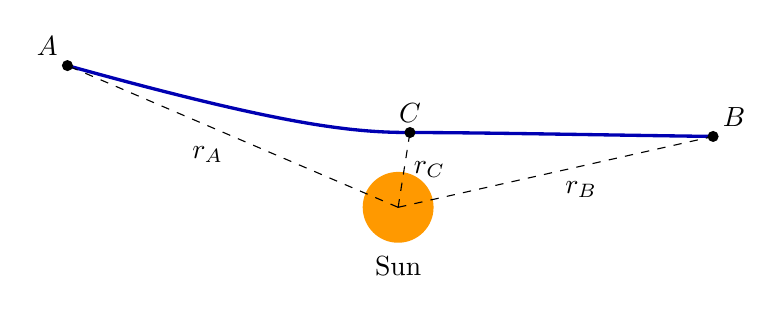
\begin{tikzpicture}[scale=1.0,>=Stealth]
  \fill[orange!80!yellow] (0,0) circle (0.45); \node[below] at (0,-0.5) {Sun};
  \coordinate (A) at (-4.2,1.8); \coordinate (B) at (4.0,0.9); \coordinate (C) at (0.15,0.95);
  \draw[very thick,blue!70!black] (A) .. controls (-1.5,1.05) and (-0.6,0.95) .. (C) .. controls (1.0,0.95) and (2.5,0.92) .. (B);
  \fill (A) circle (2pt) node[above left] {$A$};
  \fill (B) circle (2pt) node[above right] {$B$};
  \fill (C) circle (2pt) node[above] {$C$};
  \draw[dashed] (0,0) -- (A) node[midway,below left] {$r_A$};
  \draw[dashed] (0,0) -- (B) node[midway,below right] {$r_B$};
  \draw[dashed] (0,0) -- (C) node[midway,right] {$r_C$};
\end{tikzpicture}
\caption{Schematic representation of the Shapiro effect setup: a signal travels from $A$ (Earth) to $B$ (Mercury) and back, passing at a minimal distance $r_C$ from the Sun.}
\label{fig:shapiro}
\end{figure}

We assume that the entire effect takes place in a Schwarzschild space-time induced by the Sun, with the invariant length given in Schwarzschild coordinates by
\[
  \dd s^2=f(r)c^2\dd t^2-\frac{1}{f(r)}\dd r^2-r^2\big(\dd\theta^2+\sin^2\theta\,\dd\phi^2\big),\qquad f(r)=1-\frac{r_s}{r},\qquad r_s=\frac{2\GN M_\odot}{c^2}. \tag{1.1}
\]

\begin{problem}{Question 1.1}
Identify the components of the metric tensor $g_{\mu\nu}$ for the Schwarzschild geometry.
\end{problem}
\begin{solution}
From $\dd s^2=g_{\mu\nu}\dd x^\mu\dd x^\nu$ we can immediately read, in coordinates $(t,r,\theta,\phi)$,
\[
  g_{tt}=f(r)c^2,\qquad g_{rr}=-\frac{1}{f(r)},\qquad g_{\theta\theta}=-r^2,\qquad g_{\phi\phi}=-r^2\sin^2\theta,
\]
and all other $g_{\mu\nu}$'s $=0$ (the metric is diagonal). \added{With $x^0=ct$ instead, $g_{00}=f(r)$.}
\end{solution}

\begin{problem}{Question 1.2}
Let us define the Lagrangian of a test particle with mass $m=1$ (massive case) or $m=0$ (massless case) through $L=g_{\mu\nu}\frac{\dd x^\mu}{\dd\lambda}\frac{\dd x^\nu}{\dd\lambda}$, where $\lambda$ is some appropriately chosen affine parameter. Show that for a particle moving along an equatorial plane ($\theta=\pi/2$), the Lagrangian is given by
\[
  L=f(r)c^2\dot t^2-\frac{\dot r^2}{f(r)}-r^2\dot\phi^2, \tag{1.3}
\]
where the overdot denotes differentiation with respect to $\lambda$. Which could be a convenient parameter choice for $\lambda$ in the case of a massive particle? For future reference, note that $L=kc^2$, where $k=1$ for massive particles and $k=0$ for massless particles.
\end{problem}
\begin{solution}
From the Lagrangian definition,
\[
  L=f(r)c^2\dot t^2-\frac{\dot r^2}{f(r)}-r^2\dot\theta^2-r^2\sin^2\theta\,\dot\phi^2 .
\]
For movement in the equatorial plane, $\theta=\pi/2$ at all times, so $\sin^2\theta=1$ and $\dot\theta=0$:
\[
  L=f(r)c^2\dot t^2-\frac{\dot r^2}{f(r)}-r^2\dot\phi^2=\begin{cases}c^2&\text{(massive)},\\0&\text{(photons)}.\end{cases}
\]
For massive particles we typically choose $\lambda=\tau$, the proper time: then $L=\dd s^2/\dd\tau^2=c^2$. \added{(For photons $\dd\tau=0$ and $\lambda$ must be another affine parameter. Motion in the equatorial plane is consistent: the $\theta$ Euler--Lagrange equation $\frac{\dd}{\dd\lambda}(r^2\dot\theta)=r^2\sin\theta\cos\theta\,\dot\phi^2$ is satisfied by $\theta=\pi/2$, $\dot\theta=0$, and by spherical symmetry we can always orient the axes so that the motion starts in this plane.)}
\end{solution}

\begin{problem}{Question 1.3}
Starting from the Euler--Lagrange equations, show that
\[
  c^2f(r)\dot t=E,\qquad r^2\dot\phi=L_z, \tag{1.4--1.5}
\]
where $E,L_z$ are constants. What is the physical meaning of these constants? Given these results, and in the context of the problem at hand, what can we tell about conserved quantities?
\end{problem}
\begin{solution}
Euler--Lagrange equations: $\frac{\pd L}{\pd x^\alpha}-\frac{\dd}{\dd\lambda}\Big(\frac{\pd L}{\pd\dot x^\alpha}\Big)=0$. Now:
\begin{itemize}
\item $\frac{\pd L}{\pd t}=0\Rightarrow\frac{\dd}{\dd\lambda}\Big(\frac{\pd L}{\pd\dot t}\Big)=0\Rightarrow\frac{\dd}{\dd\lambda}\big(2f(r)c^2\dot t\big)=0\Rightarrow f(r)c^2\dot t=E$, where $E$ is a constant;
\item $\frac{\pd L}{\pd\phi}=0\Rightarrow\frac{\dd}{\dd\lambda}\Big(\frac{\pd L}{\pd\dot\phi}\Big)=0\Rightarrow\frac{\dd}{\dd\lambda}\big(-2r^2\dot\phi\big)=0\Rightarrow r^2\dot\phi=L_z$, where $L_z$ is a constant.
\end{itemize}
$E$ corresponds to the energy and $L_z$ to the angular momentum (per unit mass for massive particles; for $r\to\infty$, $f\to1$ and $E=c^2\,\dd t/\dd\tau=\gamma c^2$, the energy per unit mass, while $L_z=r^2\dd\phi/\dd\tau$ is the angular momentum per unit mass along the $z$ axis). From \textbf{Noether's theorem} we deduce that they are conserved along geodesics: $E$ is conserved because the metric is static (invariance under time translations $t\to t+\text{const}$, i.e.\ $\pd_t$ is a Killing vector), and $L_z$ because the metric is axially (in fact spherically) symmetric (invariance under $\phi\to\phi+\text{const}$). In the problem at hand, both the energy and the angular momentum of the photon are conserved along its whole path from $A$ to $C$ to $B$; the conservation of the total angular momentum also guarantees that the motion takes place in a plane, which justifies the choice $\theta=\pi/2$.
\end{solution}

\begin{problem}{Question 1.4}
By combining the previous questions, show that
\[
  \frac{\dot r^2}{f(r)}+\frac{L_z^2}{r^2}-\frac{E^2}{c^2f(r)}=-kc^2 . \tag{1.6}
\]
\end{problem}
\begin{solution}
From (1.3) with $L=kc^2$, and using $\dot t=\frac{E}{c^2f(r)}$, $\dot\phi=\frac{L_z}{r^2}$:
\[
  f(r)c^2\dot t^2-\frac{\dot r^2}{f(r)}-r^2\dot\phi^2=kc^2
  \ \Rightarrow\ f(r)c^2\frac{E^2}{f^2(r)c^4}-\frac{\dot r^2}{f(r)}-r^2\frac{L_z^2}{r^4}=kc^2
  \ \Rightarrow\ \frac{E^2}{c^2f(r)}-\frac{\dot r^2}{f(r)}-\frac{L_z^2}{r^2}=kc^2 ,
\]
which, multiplied by $-1$, is (1.6).
\end{solution}

\begin{problem}{Question 1.5}
From this point on, we focus our attention on massless particles. We split the calculation in two stages: from $A$ to $C$ (the point of closest approach of the signal to the Sun) and from $C$ to $B$ (and back). First, show that
\[
  \frac{1}{f(r)^3}\Big(\frac{\dd r}{\dd t}\Big)^2+\frac{c^2r_C^2}{f(r_C)\,r^2}-\frac{c^2}{f(r)}=0. \tag{1.7}
\]
\emph{Hint:} as one moves from $A$ to $C$ and then to $B$, $r$ first decreases and then increases again.
\end{problem}
\begin{solution}
We have
\[
  \frac{\dd r}{\dd\lambda}\equiv\dot r=\frac{\dd r}{\dd t}\frac{\dd t}{\dd\lambda}=\frac{\dd r}{\dd t}\dot t=\frac{\dd r}{\dd t}\frac{E}{f(r)c^2}.
\]
Then, the previous equation with $k=0$ (photons) becomes
\[
  \frac{E^2}{c^2f(r)}-\Big(\frac{\dd r}{\dd t}\Big)^2\frac{E^2}{f^3(r)c^4}-\frac{L_z^2}{r^2}=0 .
\]
Now, by the hint, $r$ reaches a minimum at $r=r_C$, so there $\frac{\dd r}{\dd t}\big|_{r=r_C}=0$, which gives
\[
  \frac{L_z^2}{r_C^2}=\frac{E^2}{f(r_C)c^2}\quad\Longrightarrow\quad L_z^2=\frac{r_C^2E^2}{f(r_C)c^2}.
\]
Substituting, we obtain
\[
  \frac{E^2}{c^2f(r)}-\Big(\frac{\dd r}{\dd t}\Big)^2\frac{E^2}{f^3(r)c^4}-\frac{r_C^2E^2}{r^2c^2f(r_C)}=0 .
\]
Multiplying by $-c^4/E^2$ we obtain
\[
  \frac{1}{f^3(r)}\Big(\frac{\dd r}{\dd t}\Big)^2+\frac{c^2r_C^2}{r^2f(r_C)}-\frac{c^2}{f(r)}=0 .
\]
\end{solution}

\begin{problem}{Question 1.6}
Show that the time, as measured in the coordinate system $(ct,r,\theta,\phi)$, that an electromagnetic signal takes to go from point $A$ to point $C$ is
\[
  t_{AC}=\frac1c\int_{r_C}^{r_A}\frac{\dd r}{\sqrt{\Big[1-\frac{f(r)}{f(r_C)}\frac{r_C^2}{r^2}\Big]f^2(r)}} . \tag{1.8}
\]
\end{problem}
\begin{solution}
From the previous question:
\begin{gather*}
  \Big(\frac{\dd r}{\dd t}\Big)^2=c^2f^2(r)-\frac{c^2r_C^2}{f(r_C)r^2}f^3(r)\\
  \ \Rightarrow\ \dd r^2=c^2f^2(r)\Big[1-\frac{r_C^2}{r^2}\frac{f(r)}{f(r_C)}\Big]\dd t^2\\
  \ \Rightarrow\ \dd t=\pm\frac1c\frac{\dd r}{\sqrt{\Big(1-\frac{r_C^2}{r^2}\frac{f(r)}{f(r_C)}\Big)f^2(r)}} .
\end{gather*}
From $A$ to $C$, $r$ decreases while $t$ increases, so we take the minus sign: $t_{AC}=-\frac1c\int_{r_A}^{r_C}(\dots)=\frac1c\int_{r_C}^{r_A}(\dots)$, i.e.
\[
  t_{AC}=\frac1c\int_{r_C}^{r_A}\frac{\dd r}{\sqrt{\Big(1-\frac{r_C^2}{r^2}\frac{f(r)}{f(r_C)}\Big)f^2(r)}} .
\]
\added{The integrand diverges at $r=r_C$ like $(r-r_C)^{-1/2}$, which is integrable.}
\end{solution}

\begin{problem}{Question 1.7}
Keeping only first order terms in the $\epsilon\equiv r_s/r_C$ and $\delta\equiv r_s/r$ expansion, one can show that the integrand of the last expression can be written as
\[
  \frac{1}{\sqrt{\Big[1-\frac{f(r)}{f(r_C)}\frac{r_C^2}{r^2}\Big]f^2(r)}}\simeq\frac{r}{\sqrt{r^2-r_C^2}}\Big(1+\frac{r_s}{r}+\frac{r_sr_C}{2r(r+r_C)}\Big). \tag{1.9}
\]
The question is: are we allowed to make this approximation? Justify your answer numerically.
\end{problem}
\begin{solution}
Yes, because $r_s$ lies deep inside the Sun, and the signal never gets closer to the centre of the Sun than its radius: $r\ge r_C\ge R_\odot$. \added{Numerically,
\[
  r_s=\frac{2\GN M_\odot}{c^2}=\frac{2\times6.67\times10^{-11}\times1.99\times10^{30}}{(3.00\times10^8)^2}\,\mathrm m\simeq2.95\,\mathrm{km},\qquad R_\odot\simeq6.96\times10^5\,\mathrm{km},
\]
so $\delta\le\epsilon\le r_s/R_\odot\simeq4.2\times10^{-6}$. The neglected second-order terms are of order $\epsilon^2\sim10^{-11}$, completely negligible (they would contribute $\sim10^{-11}\times$ the travel time $\sim10^{-9}$\,s, to be compared with a relativistic delay of $\sim10^{-4}$\,s).}

\added{\textit{Derivation of (1.9).} To first order, $\frac{f(r)}{f(r_C)}=\frac{1-\delta}{1-\epsilon}\simeq1+\epsilon-\delta$, with $\epsilon-\delta=r_s\big(\frac1{r_C}-\frac1r\big)=\frac{r_s(r-r_C)}{rr_C}$. Hence
\[
  1-\frac{r_C^2}{r^2}\frac{f(r)}{f(r_C)}\simeq\frac{r^2-r_C^2}{r^2}-\frac{r_C^2}{r^2}\frac{r_s(r-r_C)}{rr_C}
  =\frac{r^2-r_C^2}{r^2}\Big[1-\frac{r_sr_C}{r(r+r_C)}\Big],
\]
using $r^2-r_C^2=(r-r_C)(r+r_C)$. Then, with $(1-x)^{-1/2}\simeq1+x/2$ and $1/f(r)\simeq1+r_s/r$,
\[
  \frac{1}{f(r)}\Big[1-\frac{r_C^2}{r^2}\frac{f(r)}{f(r_C)}\Big]^{-1/2}\simeq\Big(1+\frac{r_s}{r}\Big)\frac{r}{\sqrt{r^2-r_C^2}}\Big(1+\frac{r_sr_C}{2r(r+r_C)}\Big)
  \simeq\frac{r}{\sqrt{r^2-r_C^2}}\Big(1+\frac{r_s}{r}+\frac{r_sr_C}{2r(r+r_C)}\Big).
\]
Note that the expansion is uniform: the singular factor $\sqrt{r^2-r_C^2}$ has been factorised exactly, and only the small corrections were expanded.}
\end{solution}

\begin{problem}{Question 1.8}
In this approximation, show that the time needed for the light signal to travel from $A$ to $C$ is given by
\[
  t_{AC}=\frac1c\sqrt{r_A^2-r_C^2}+\frac{r_s}{c}\ln\left(\frac{r_A+\sqrt{r_A^2-r_C^2}}{r_C}\right)+\frac{r_s}{2c}\sqrt{\frac{r_A-r_C}{r_A+r_C}} . \tag{1.10}
\]
What would the corresponding result be in the absence of any relativistic effects?
\end{problem}
\begin{solution}
We have:
\begin{gather*}
  t_{AC}\simeq\frac1c\int_{r_C}^{r_A}\dd r\left[\frac{r}{\sqrt{r^2-r_C^2}}\Big(1+\frac{r_s}{r}+\frac{r_sr_C}{2r(r+r_C)}\Big)\right]\\
  =\frac1c\int_{r_C}^{r_A}\Big[\frac{r}{\sqrt{r^2-r_C^2}}+\frac{r_s}{\sqrt{r^2-r_C^2}}+\frac{r_sr_C}{2(r+r_C)\sqrt{r^2-r_C^2}}\Big]\dd r .
\end{gather*}
Using the three useful integrals (0.1)--(0.3) with $a=r_C$:
\begin{align*}
  t_{AC}&=\frac1c\Big[\sqrt{r^2-r_C^2}\Big]_{r_C}^{r_A}+\frac{r_s}{c}\left[\ln\frac{r+\sqrt{r^2-r_C^2}}{r_C}\right]_{r_C}^{r_A}+\frac{r_s}{2c}\left[\sqrt{\frac{r-r_C}{r+r_C}}\right]_{r_C}^{r_A}\\
  &=\frac1c\sqrt{r_A^2-r_C^2}+\frac{r_s}{c}\ln\left[\frac{r_A+\sqrt{r_A^2-r_C^2}}{r_C}\right]+\frac{r_s}{2c}\sqrt{\frac{r_A-r_C}{r_A+r_C}},
\end{align*}
since all three primitives vanish at $r=r_C$ ($\ln(r_C/r_C)=0$). In the absence of relativistic effects ($r_s\to0$), only the first term would survive: $t_{AC}^{\rm flat}=\frac1c\sqrt{r_A^2-r_C^2}$, the time needed to travel at speed $c$ along the straight segment from $A$ to $C$ (Pythagoras).
\end{solution}

\begin{problem}{Question 1.9}
Lastly, consider the total travel time from $A$ to $B$ and back. Show that the maximal time delay with respect to the result that we would obtain in the absence of any relativistic effects can be approximated by
\[
  \delta t_{\max}=\frac{4\GN M_\odot}{c^3}\left(1+\ln\frac{4r_Ar_B}{R_\odot^2}\right), \tag{1.11}
\]
where $M_\odot$ and $R_\odot$ are the mass and the radius of the Sun, respectively.
\end{problem}
\begin{solution}
The total travel time is $t_{\rm tot}=2t_{AC}+2t_{BC}$ (from $A$ to $C$ to $B$ and back), where $t_{BC}$ is given by (1.10) with $r_A\to r_B$. By dropping the Newtonian part, the delay is
\[
  \delta t=\frac{2r_s}{c}\left[\ln\frac{\big(r_A+\sqrt{r_A^2-r_C^2}\big)\big(r_B+\sqrt{r_B^2-r_C^2}\big)}{r_C^2}+\frac12\sqrt{\frac{r_A-r_C}{r_A+r_C}}+\frac12\sqrt{\frac{r_B-r_C}{r_B+r_C}}\right].
\]
It is a decreasing function of $r_C$, so it is maximal when $r_C$ is as small as possible, i.e.\ when the signal grazes the Sun, $r_C=R_\odot$ (planet $B$ near superior conjunction). Approximating $r_{A/B}\pm R_\odot\simeq r_{A/B}$ and $r_{A/B}^2-R_\odot^2\simeq r_{A/B}^2$ (since $r_A,r_B\gg R_\odot$), we get:
\[
  \delta t_{\max}=\frac1c\Big[2r_s+2r_s\ln(4r_Ar_B)-2r_s\ln(R_\odot^2)\Big]=\frac{2r_s}{c}\Big[1+\ln\frac{4r_Ar_B}{R_\odot^2}\Big]=\frac{4\GN M_\odot}{c^3}\Big[1+\ln\frac{4r_Ar_B}{R_\odot^2}\Big].
\]
\added{(The two square roots tend to $1$ each, giving $\frac12+\frac12=1$, and $\ln\frac{(2r_A)(2r_B)}{R_\odot^2}=\ln\frac{4r_Ar_B}{R_\odot^2}$.)

\textit{Numerical estimate} for Earth ($r_A=1\,\mathrm{AU}=1.50\times10^{11}$\,m) and Mercury ($r_B=5.79\times10^{10}$\,m): $\frac{4r_Ar_B}{R_\odot^2}\simeq7.2\times10^4$, $\ln(\dots)\simeq11.2$; with $\GN M_\odot/c^3\simeq4.93\,\mu$s,
\[
  \delta t_{\max}\simeq4\times4.93\,\mu\mathrm s\times12.2\simeq240\,\mu\mathrm s ,
\]
a delay that was measured by I.~Shapiro and collaborators with radar echoes from Mercury and Venus, in agreement with GR.}
\end{solution}

\subsection{Exercise 2: a perfect fluid star}

In this exercise we study some aspects of a simple model describing the interior of a star. Similarly to the derivation of the Schwarzschild metric, we assume that the entire problem is characterised by spherical symmetry and that the metric is static. Under these assumptions, the general form of the line element is
\[
  \dd s^2=A(r)\dd t^2-B(r)\dd r^2-r^2\big(\dd\theta^2+\sin^2\theta\,\dd\phi^2\big), \tag{2.1}
\]
where $A(r)$, $B(r)$ can be determined by solving the Einstein field equations in the interior of the object once the form of the stress--energy--momentum tensor is specified. On top of the previous assumptions, we assume that the interior of the star behaves like a perfect fluid of proper mass density $\rho(r)$ and isotropic pressure $p(r)$ in the instantaneous rest frame of the fluid. For a static matter distribution, both $\rho$ and $p$ only depend on $r$. (Units $c=1$; the approximation adopted here leads to the Tolman--Oppenheimer--Volkoff equation of stellar structure.)

\begin{problem}{Question 2.1}
First, let us ignore the specific configuration that we are considering. Show that, in full generality, the Einstein field equations can be written under the alternative form
\[
  R_{\mu\nu}=\kappa\Big(T_{\mu\nu}-\frac12Tg_{\mu\nu}\Big), \tag{2.2}
\]
where $\kappa\equiv8\pi\GN$ and $T\equiv T^\mu{}_\mu$ is the trace of the stress--energy--momentum tensor.
\end{problem}
\begin{solution}
The Einstein equations are $R_{\mu\nu}-\frac12Rg_{\mu\nu}=\kappa T_{\mu\nu}$. Multiplying by $g^{\alpha\mu}$:
\[
  g^{\alpha\mu}R_{\mu\nu}-\frac12Rg^{\alpha\mu}g_{\mu\nu}=\kappa g^{\alpha\mu}T_{\mu\nu}\ \Rightarrow\ R^\alpha{}_\nu-\frac12R\delta^\alpha{}_\nu=\kappa T^\alpha{}_\nu .
\]
Setting $\alpha=\nu$ (and summing): $R^\nu{}_\nu-\frac12R\delta^\nu{}_\nu=\kappa T^\nu{}_\nu\Rightarrow R-\frac42R=\kappa T\Rightarrow R=-\kappa T$. Then the EFE become
\[
  R_{\mu\nu}+\frac12\kappa Tg_{\mu\nu}=\kappa T_{\mu\nu}\quad\Longrightarrow\quad R_{\mu\nu}=\kappa\Big(T_{\mu\nu}-\frac12Tg_{\mu\nu}\Big).
\]
\end{solution}

\begin{problem}{Question 2.2}
Show that, in this case, Eq.~(2.2) takes the form
\[
  R_{\mu\nu}=\kappa\Big[(\rho+p)u_\mu u_\nu-\frac12(\rho-p)g_{\mu\nu}\Big]. \tag{2.3}
\]
\emph{Hint:} note that $u^\mu u_\mu=1$.
\end{problem}
\begin{solution}
For a perfect fluid $T_{\mu\nu}=(\rho+p)u_\mu u_\nu-pg_{\mu\nu}$. Multiplying by $g^{\mu\nu}$:
\[
  T\equiv g^{\mu\nu}T_{\mu\nu}=(\rho+p)\underbrace{g^{\mu\nu}u_\mu u_\nu}_{u^\mu u_\mu=1}-p\underbrace{g^{\mu\nu}g_{\mu\nu}}_{\delta^\mu{}_\mu=4}=(\rho+p)-4p=\rho-3p .
\]
Then the EFE become
\[
  R_{\mu\nu}=\kappa\Big[(\rho+p)u_\mu u_\nu-pg_{\mu\nu}-\frac12(\rho-3p)g_{\mu\nu}\Big]=\kappa\Big[(\rho+p)u_\mu u_\nu-\frac12(\rho-p)g_{\mu\nu}\Big].
\]
\end{solution}

\begin{problem}{Question 2.3}
Given the geometry of the problem, the only non-zero components of the Ricci tensor read
\begin{align*}
  R_{tt}&=\frac{A''}{2B}+\frac{A'}{rB}-\frac{(A')^2}{4AB}-\frac{A'B'}{4B^2},\qquad
  R_{rr}=-\frac{A''}{2A}+\frac{B'}{rB}+\frac{(A')^2}{4A^2}+\frac{A'B'}{4AB},\\
  R_{\theta\theta}&=\frac{B-1}{B}-\frac{rA'}{2AB}+\frac{rB'}{2B^2},\qquad R_{\phi\phi}=\sin^2\theta R_{\theta\theta}, \tag{2.4}
\end{align*}
where the primes denote differentiation with respect to $r$. With this as a given, show that the covariant components of the fluid 4-velocity read $u_\mu=\sqrt A\,(1,0,0,0)$. \emph{Hint:} Eq.~(2.3) and the structure of the Ricci tensor have implications for the velocity components.
\end{problem}
\begin{solution}
From the expressions for $R_{\mu\nu}$ we see that all off-diagonal elements vanish. Then, from the result of the previous question, we have for instance
\[
  R_{0i}=0\ \Rightarrow\ \kappa\Big[(\rho+p)u_0u_i-\frac12(\rho-p)\underbrace{g_{0i}}_{=0}\Big]=0\ \Rightarrow\ u_0u_i=0
\]
(assuming $\rho+p\neq0$, which holds for ordinary matter). But $u_0\neq0$ (otherwise $u^\mu u_\mu=g^{ij}u_iu_j\le0$ could not equal $1$: a time-like vector must have a non-zero time component), hence $u_i=0$: the fluid is at rest in these coordinates, as expected for a static star. \added{(The equations $R_{ij}=0$ for $i\neq j$ are then automatically satisfied.)}

At the same time, $u^\mu u_\mu=1\Rightarrow g^{\mu\nu}u_\mu u_\nu=1\overset{u_i=0}{\Longrightarrow}g^{00}u_0^2=1\Rightarrow\frac{u_0^2}{A(r)}=1\Rightarrow u_0=\sqrt{A(r)}$ (choosing the future-directed solution). Therefore $u_\mu=\sqrt{A(r)}\,(1,0,0,0)$ \added{and $u^\mu=g^{\mu\nu}u_\nu=\frac{1}{\sqrt{A}}(1,0,0,0)$}.
\end{solution}

\begin{problem}{Question 2.4}
Show that the non-zero (diagonal) components of the Ricci tensor read
\[
  R_{tt}=\frac12\kappa(\rho+3p)A,\qquad R_{rr}=\frac12\kappa(\rho-p)B,\qquad R_{\theta\theta}=\frac12\kappa(\rho-p)r^2,\qquad R_{\phi\phi}=\sin^2\theta R_{\theta\theta}. \tag{2.6--2.9}
\]
\end{problem}
\begin{solution}
We found $R_{\mu\nu}=\kappa\big[(\rho+p)u_\mu u_\nu-\frac12(\rho-p)g_{\mu\nu}\big]$ with $u_\mu=\sqrt{A}(1,0,0,0)$, so $u_tu_t=A$ and $u_\mu u_\nu=0$ otherwise. With $g_{tt}=A$, $g_{rr}=-B$, $g_{\theta\theta}=-r^2$, $g_{\phi\phi}=-r^2\sin^2\theta$:
\begin{align*}
  R_{tt}&=\kappa\Big[(\rho+p)A-\frac12(\rho-p)A\Big]=\frac\kappa2\big[\rho+3p\big]A(r),\\
  R_{rr}&=\kappa\Big[0-\frac12(\rho-p)(-B)\Big]=+\frac\kappa2(\rho-p)B(r),\\
  R_{\theta\theta}&=\kappa\Big[0-\frac12(\rho-p)(-r^2)\Big]=\frac\kappa2(\rho-p)r^2,\\
  R_{\phi\phi}&=\frac\kappa2(\rho-p)r^2\sin^2\theta=\sin^2\theta R_{\theta\theta}.
\end{align*}
\end{solution}

\begin{problem}{Question 2.5}
Show that $B(r)$ satisfies the differential equation
\[
  \Big(1-\frac1B\Big)+\frac{rB'}{B^2}=\kappa r^2\rho(r). \tag{2.10}
\]
\emph{Hint:} the easiest way is by considering the combination $R_{tt}/A+R_{rr}/B+2R_{\theta\theta}/r^2$.
\end{problem}
\begin{solution}
We have, from the matter side (Question 2.4):
\[
  \frac{R_{tt}}{A}+\frac{R_{rr}}{B}+\frac{2R_{\theta\theta}}{r^2}=\frac12\kappa(\rho+3p)+\frac12\kappa(\rho-p)+\kappa(\rho-p)=2\kappa\rho .\tag{I}
\]
At the same time, from the general geometric expressions (2.4) we have:
\begin{align*}
  \frac{R_{tt}}{A}+\frac{R_{rr}}{B}+\frac{2R_{\theta\theta}}{r^2}
  &=\cancel{\frac{A''}{2AB}}+\bcancel{\frac{A'}{rAB}}-\xcancel{\frac{(A')^2}{4A^2B}}-\frac{A'B'}{4AB^2}
  -\cancel{\frac{A''}{2AB}}+\frac{B'}{rB^2}+\xcancel{\frac{(A')^2}{4A^2B}}+\frac{A'B'}{4AB^2}\\
  &\quad+\frac{2(B-1)}{r^2B}-\bcancel{\frac{2A'}{2rAB}}+\frac{2B'}{2rB^2}
  =\frac{2B'}{rB^2}+\frac{2(B-1)}{r^2B}.\tag{II}
\end{align*}
(The terms $\pm\frac{A'B'}{4AB^2}$ cancel as well.) From (I) and (II):
\[
  \frac{B-1}{r^2B}+\frac{B'}{rB^2}=\kappa\rho\quad\Longrightarrow\quad\Big(1-\frac1B\Big)+\frac{rB'}{B^2}=\kappa r^2\rho .
\]
\end{solution}

\begin{problem}{Question 2.6}
Show that this result leads to
\[
  B(r)=\Big[1-\frac{2\GN m(r)}{r}\Big]^{-1}, \tag{2.11}
\]
where we have defined the function
\[
  m(r)=4\pi\int_0^r\rho(r')r'^2\dd r'. \tag{2.12}
\]
\emph{Hint:} note that the left-hand side of Eq.~(2.10) can be written as a derivative.
\end{problem}
\begin{solution}
We have:
\[
  \frac{\dd}{\dd r}\Big[r\Big(1-\frac1B\Big)\Big]=\Big(1-\frac1B\Big)+r\frac{B'}{B^2}=\kappa r^2\rho .
\]
Integrating from $0$ to $r$ \added{(the boundary term at $r=0$ vanishes, since $B(0)$ must be finite for the geometry to be regular at the centre; in fact $B(0)=1$, local flatness)}:
\[
  r\Big(1-\frac1B\Big)=\int_0^r8\pi\GN r'^2\rho(r')\dd r'=2\GN\underbrace{4\pi\int_0^rr'^2\rho(r')\dd r'}_{=m(r)}=2\GN m(r).
\]
Hence
\[
  1-\frac1B=\frac{2\GN m(r)}{r}\ \Rightarrow\ \frac1B=1-\frac{2\GN m(r)}{r}\ \Rightarrow\ B(r)=\Big[1-\frac{2\GN m(r)}{r}\Big]^{-1}.
\]
\added{Outside the star ($r>R$, $\rho=0$), $m(r)=m(R)\equiv M$ is constant and $B=(1-2\GN M/r)^{-1}$: we recover exactly the Schwarzschild $g_{rr}$, so $M=m(R)$ is the mass measured by distant observers (e.g.\ from Kepler orbits).}
\end{solution}

\begin{problem}{Question 2.7}
One might be tempted to interpret the function (2.12) as representing the mass contained within a coordinate radius $r$. This interpretation is, however, not exactly accurate.
\begin{enumerate}[label=\roman*)]
\item Why is this interpretation incorrect? Which would, instead, be the correct expression for the physical (invariant) ``mass'' $\tilde m(r)$ contained within a coordinate radius $r$?
\item Based on your answers and noting that, however, it is $m$ and not $\tilde m$ that appears in the radial metric coefficient $B(r)$, can you think what the difference between these two masses corresponds to physically?
\end{enumerate}
\end{problem}
\begin{solution}
\textbf{i)} The definition of $m(r)$ uses the \emph{flat-space} volume element $4\pi r'^2\dd r'$, which is not the physical (invariant) volume in the curved geometry \added{(and $r$ is not the proper radial distance)}. The physical (invariant) volume element in space, at fixed $t$, is given by the spatial metric $\dd l^2=B\,\dd r^2+r^2\dd\theta^2+r^2\sin^2\theta\dd\phi^2$:
\[
  \dd V^3=\sqrt{|\det(g_{ij})|}\,\dd r\,\dd\theta\,\dd\phi=\sqrt{B(r)r^4\sin^2\theta}\,\dd r\,\dd\theta\,\dd\phi=\sqrt{B(r)}\,r^2\sin\theta\,\dd r\,\dd\theta\,\dd\phi .
\]
The physical (invariant) mass contained in a ``sphere'' of coordinate radius $r$ is then
\[
  \tilde m(r)\equiv m_{\rm phys}(r)=\int_{-1}^{1}\dd(\cos\theta)\int_0^{2\pi}\dd\phi\int_0^r\sqrt{B(r')}\,r'^2\rho(r')\dd r'=4\pi\int_0^r\sqrt{B(r')}\,r'^2\rho(r')\dd r'\neq m(r).
\]
Since $B>1$ inside the star, $\tilde m(r)>m(r)$.

\textbf{ii)} The difference corresponds to the \textbf{gravitational binding energy} of the star. $\tilde m$ is the sum of the masses (rest mass plus internal energy) of all the fluid elements; $m=m(R)$ is the total mass--energy of the star as felt by an external observer, which includes the (negative) gravitational potential energy. \added{Indeed, in the weak-field limit $\sqrt B\simeq1+\frac{\GN m(r)}{r}$, so
\[
  \tilde m-m\simeq4\pi\GN\int_0^R\frac{m(r)}{r}\rho(r)r^2\dd r=\int_0^R\frac{\GN m(r)\,\dd m}{r},\qquad\dd m=4\pi r^2\rho\,\dd r,
\]
which is exactly the Newtonian binding energy (with $c=1$): the energy needed to disperse the star's material to infinity, built shell by shell, each shell $\dd m$ being brought from infinity in the field of the mass $m(r)$ already present. Assembling the star releases this energy, so the gravitating mass $m$ is smaller than the sum $\tilde m$ of the masses of its constituents.}
\end{solution}

\end{document}
